\chapter{Approaches for developing ontologies}
\label{ch:development_approaches}

% TODO criteria about how to "rate" approaches

\section{Ontology 101}

\section{Methodology by Noy and McGuinness}

\section{Methodology by Uschold and King}

\section{Methodology by Grüninger and Fox}

\section{METHONTOLOGY}

% TODO mention IEEE software life cycle paper referenced in \cite{MethontologyLegal}?
The authors of the article introducing the approach named \methontology, Gómez-Pérez et al., perceived absence of a clear engineering approach towards building ontology from scratch \cite{Methontology}. Hence, Gómez-Pérez et al. described a process for developing ontologies and specified a life cycle for ontologies. Based upon that, they specified \methontology as a straight-forward engineering approach for building ontologies.

% TODO reference more papers?
There are several papers describing how to apply \methontology on certain domains \cite{MethontologyLegal} \cite{MethontologyChemical}. While the overall approach is the same in all of these articles, there are slight differences in the details of each step. This section describes the steps used in chapter \ref{ch:thinkhomeweather_ontology}. Thus, it differs slightly from the steps described in \cite{Methontology}.

\subsection{Ontology development process and life cycle}

The ontology development process as used by Gómez-Pérez et al. divides ontology development into the following activities that need to be performed \cite{Methontology}:

% TODO emphazise steps as in \cite{Methontology}?
% TODO remove 'must's
\begin{itemize}
  \item The whole process must be planned regarding which tasks need to be done, how they will be arranged and which resources they require.
  \item The purpose, intended uses and end-users must be specified in an ontologies requirements specification document.
  \item Knowledge about the ontology's domain must be acquired.
  \item The knowledge previously acquired must be conceptualized in a conceptual model describing the problem and its solution.
  \item This conceptual model will then be formalized.
  \item As ontologies are build to be reused, as many existing ontologies as possible will be integrated into the new ontology.
  \item The ontology will then be implemented using a formal language.
  \item The implemented ontology will be evaluated in order to ensure it fits the requirements specified previously.
  \item The whole work must be documented well.
  \item There are always things that can be modified in an ontology, therefore maintenance is necessary.
\end{itemize}

% TODO placement?
\begin{figure}
  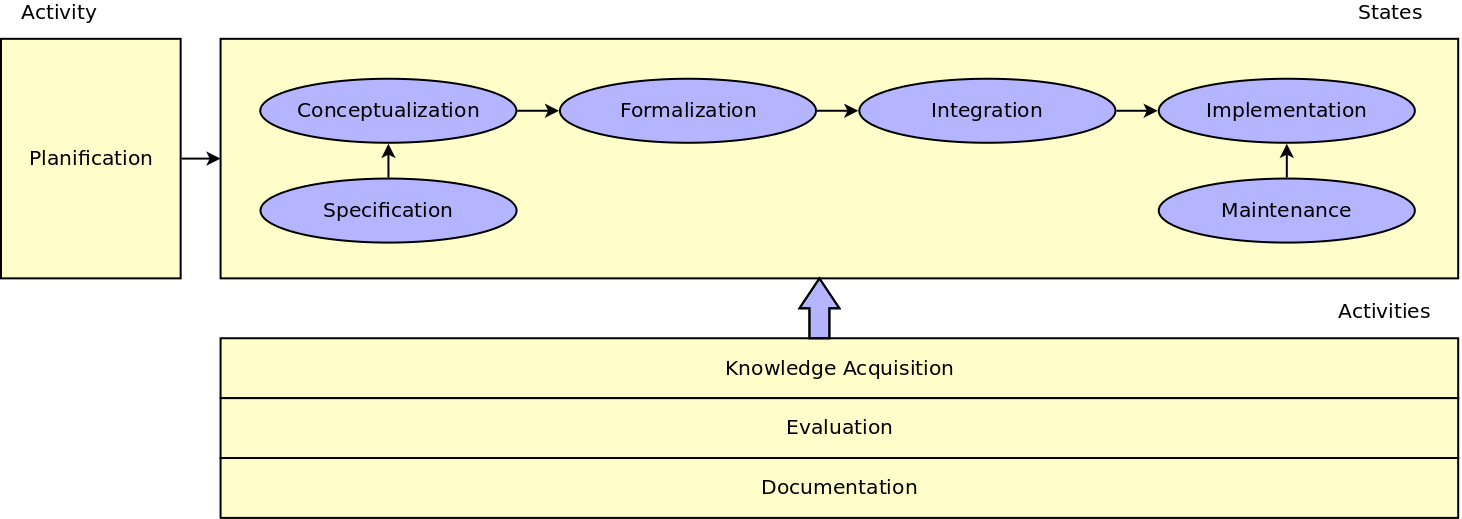
\includegraphics[width=\textwidth]{figures/ontology_lifecycle.png}
  \caption{States and activities in the life cycle of an ontology according to \methontology \cite{Methontology}}
  \label{fig:methontology1}
\end{figure}

As seen in figure \ref{fig:methontology1}, these groups are split into \emph{planification} that must be performed at the very beginning of development, a \emph{set of stages} (consisting of \emph{specification}, \emph{conceptualization}, \emph{formalization}, \emph{integration}, \emph{implementation} and \emph{maintenance}) through which the ontology moves during its life and some activities (\emph{knowledge acquisition}, \emph{documentation} and \emph{evaluation}) that are performed throughout the whole development process in parallel to the stages.

Differently to what is shown in figure \ref{fig:methontology1}, \methontology follows an \emph{evolving} life cycle model which allows the ontology to grow according to its needs. Whenever it is necessary, pieces of the ontology can be added, modified and deleted. Thus, one state does not have to be completely finished before the next state is begun. The ontology will cycle through each state numerous times until the ontology fits the requirements and the results of each step correspond to each other.

\subsection{METHONTOLOGY}
\label{sec:methontology}

This section describes \methontology as a well-defined approach to perform all activities mentioned above.

Only the idea behind \methontology is described; for the application of \methontology refer to chapter \ref{ch:thinkhomeweather_ontology} where it is used to create the \thinkhomeweather ontology.

\subsubsection{Specification}

As \methontology specifies a clear structure for developing an ontology, the planning step may be omitted. Hence, \emph{specification} is the first step of developing an ontology from scratch. During \emph{specification}, an ontology specification document is produced. That document is written in natural language using a set of intermediate representations or using competence questions. It should include the following:

\begin{itemize}
  \item The purpose of the ontology, its intended uses, scenarios of use, end-users etc.
  \item The level of formality (highly informal, semi-informal, semi-formal or rigorously formal). % TODO reference to Uschuld & Gruninger 1996
  \item The scope which includes the set of terms to be represented, its characteristics and its granularity.
\end{itemize}

A good ontology specification document has the following properties:

\begin{itemize}
  \item \textbf{Consision}: Every term is relevant and there are no duplicated or irrelevant terms.
  \item \textbf{Partial completeness}: % TODO specify?
  \item \textbf{Consistency}: All terms and their meanings make sense in the domain.
\end{itemize}

\subsubsection{Knowledge Acquisition}

Most of knowledge acquisition is done simultanously with the \emph{specification} phase. It is one of the most important activities and needs to be performed thoroughly as most other activities depend heavily on it.

Sources of knowledge are experts, books, handbooks, figures, tables and even other ontologies. Knowledge will be collected using techniques such as brainstorming, interviews, formal and informal analysis of texts and knowledge acquisition tools.

\subsubsection{Conceptualization}

% TODO placement?
\begin{figure}
  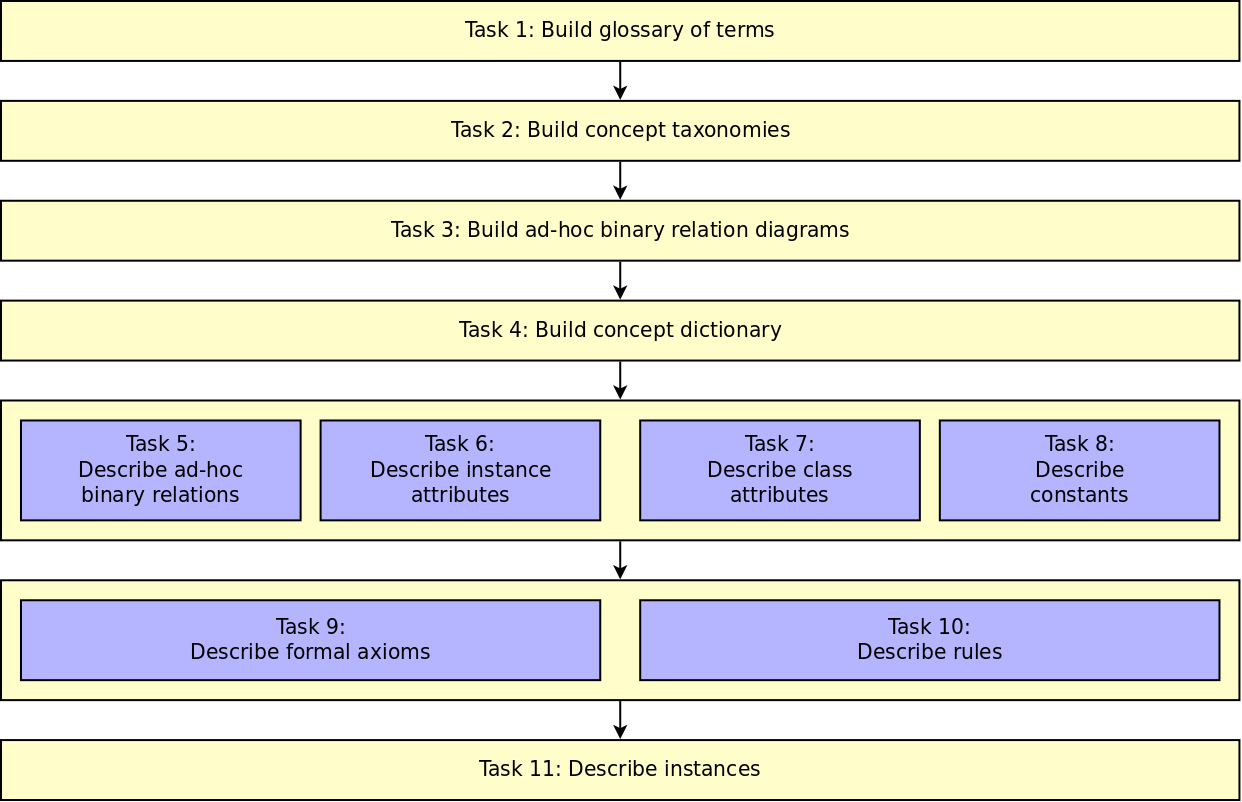
\includegraphics[width=\textwidth]{figures/methontology_tasks.png}
  \caption{Tasks of the conceptualization activity according to \methontology \cite{MethontologyLegal}}
  \label{fig:methontology2}
\end{figure}

The state of \emph{conceptualization} consists of several tasks as shown in figure \ref{fig:methontology2} \cite{MethontologyLegal}. Again, the figure shows the tasks in a sequential manner. However, as \methontology uses an evolutional process model, the steps will be performed numerous times.

% TODO these sections do not relate to the sections in the next chapter?!
\paragraph{Task 1: Glossary of Terms}

At first, the ontologist builds a \emph{Glossary of Terms}. This glossary includes all the relevant terms of the domain (concepts, instances, attributes, relations etc.). It can be built as a table having the columns \emph{name}, \emph{synonyms}, \emph{acronyms}, \emph{description} (for a natural language description of the term) and \emph{type} (specifying whether the term is a concept, an instance, an attribute, a relation etc.).

\paragraph{Task 2: Concept Taxonomies}

When the glossary of terms contains a sizable number of concepts, these ontologies will be arranged one or more taxonomies that define the concept hierarchy. It is advisable to display the taxonomies in several diagrams.

% TODO reference Frame Ontology and OKBC Ontology
\methontology proposes the use of four taxonomic relations:
% TODO description
\begin{enumerate}
  \item \textbf{Subclass-Of}
  \item \textbf{Disjoint-Decomposition}
  \item \textbf{Exhaustive-Decomposition}
  \item \textbf{Partition}
\end{enumerate}

% TODO error check?

\paragraph{Task 3: Ad-hoc binary relation diagrams}

In the next step, \emph{ad-hoc binary relation diagrams} are created. This diagrams show all ad-hoc relationships between concepts of the same (or different) concept taxonomy.

% TODO error check

\paragraph{Task 4: Concept dictionary}

The \emph{concept dictionary} contains all domain concepts together with their relations, their instances and their class and instance attributes. All information from the previous steps That dictionary will again be built as a table having appropriate columns.

% TODO error check

\paragraph{Task 5: Ad-hoc binary relation details}

In this step, for all ad-hoc binary relations details will be specified in a tabular manner. The resulting table will have a row for each relation and columns named \emph{relation name}, \emph{source concept}, \emph{source cardinality (max)}, \emph{target concept}, \emph{inverse relation}.

% TODO error check

\paragraph{Task 6: Instance attributes}

This step yields an \emph{instance attributes table}. That is a table of all \emph{instance attributes} that are listed in the concept dictionary. Each row contains the description of one instance attribute. An instance attribute is an attribute that describes an instance of a concept. Its value may be different for each instance of the concept. The columns of the table are \emph{attribute name}, \emph{concept name}, \emph{value type} (\emph{Integer}, \emph{Float}, \emph{String}, etc.), \emph{value range}, \emph{minimum cardinality} and \emph{maximum cardinality}. Additionally, the following information may be specified: instance attributes, class attributes and constants used to infer values of the attribute; attributes that can be inferred using values of this attribute; formulae or rules that allow inferring values of the attribute; and references used to define the attribute.

\paragraph{Task 7: Class attributes}

All class attributes that are listed in the concept dictionary are described in detail in the \emph{class attributes table}. Each row describes one class attribute. The columns will be \emph{name}, \emph{concept name} (i.e. the name of the concept where the attribute is defined), \emph{value type}, \emph{value(s)}, \emph{minimum cardinality} and \emph{maximum cardinality}. Additionally, all information about related instance attributes, class attributes, constants, rules and formulae may be specified that are specified in the instance attribute as well.

\paragraph{Task 8: Constants}

In this step, the \emph{constants table} is created that specifies details about all the constants listed in the glossary of terms. For each constant the following is specified: name, value type, value, the measurement unit for numerical constants and the attributes that can be inferred using the constant.

\paragraph{Task 9: Formal axioms}

% TODO

\paragraph{Task 10: Rules}

% TODO

\paragraph{Task 11: Instances}

% TODO

\subsubsection{Integration}

As ontologies are built for reuse and the wheel shall not be reinvented during the creation of a new ontology, the ontologist searches for existing ontologies. The goal is to import ontologies that already define terms that are part of the conceptualization of the ontology currently being developed.

\subsubsection{Implementation}

% TODO references
The task of implementation requires an environment that supports the ontologies selected in the integration step. Features that should be provided by such an environment are

% TODO make description more detailled?
\begin{itemize}
  \item a lexical and syntactic analyzer to guarantee the absence of lexical and syntactic errors,
  \item an editor for adding, modifying and removing definitions,
  \item a browser for inspecting the library of ontologies and their definitions,
  \item a searcher for looking for the most appropriate definitions,
  \item evaluators for detecting incompleteness, inconsistencies and redundant knowledge and
  \item an automatic maintainer for managing the inclusion, removal or modification of existing definitions.
\end{itemize}
 

In the case of the \thinkhomeweather ontology an \emph{OWL} ontology is created using \emph{Protege} together with the Pellet reasoner.

\subsubsection{Evaluation}

% TODO

\subsubsection{Documentation}

Due to its approach that generates a lot of documents, \methontology includes documentation as an activity that is done during the whole ontology development process. That means that once you are finished building an ontology using \methontology, its documentation will be complete as well.

\section{Software engineering approach by De Nicola, Missikoff and Navigli}

\section{Conclusion}

The previous chapters gave detailled insights into some popular approaches of developing ontologies from scratch. Table ? summarizes some of the key charasteristics of these approaches.

% TODO insert table

Considering the characteristics of the development approaches, \methontology was chosen for building the \thinkhomeweather ontology. Thus, \methontology was discussed more thoroughly than the other approaches. The main reasons for that decision were:

% TODO
\begin{itemize}
  \item Some reason.
  \item Some more reason.
  \item And yet another reason.
\end{itemize}

Chapter \ref{ch:thinkhomeweather_ontology} describes the process of building the \thinkhomeweather ontology in detail.